\documentclass{article}

\usepackage{graphicx}
\usepackage{tikz}
\usepackage{tikzsymbols}
\usetikzlibrary{calc,patterns,shapes.geometric}
\pagestyle{empty}
\usepackage[margin=0pt]{geometry}
\geometry{papersize={14in,12in}}

\def\centerarc[#1](#2)(#3:#4:#5){\draw[#1] ($(#2)+({#5*cos(#3)},{#5*sin(#3)})$) arc (#3:#4:#5);}

\begin{document}
	\begin{figure}
		\centering
		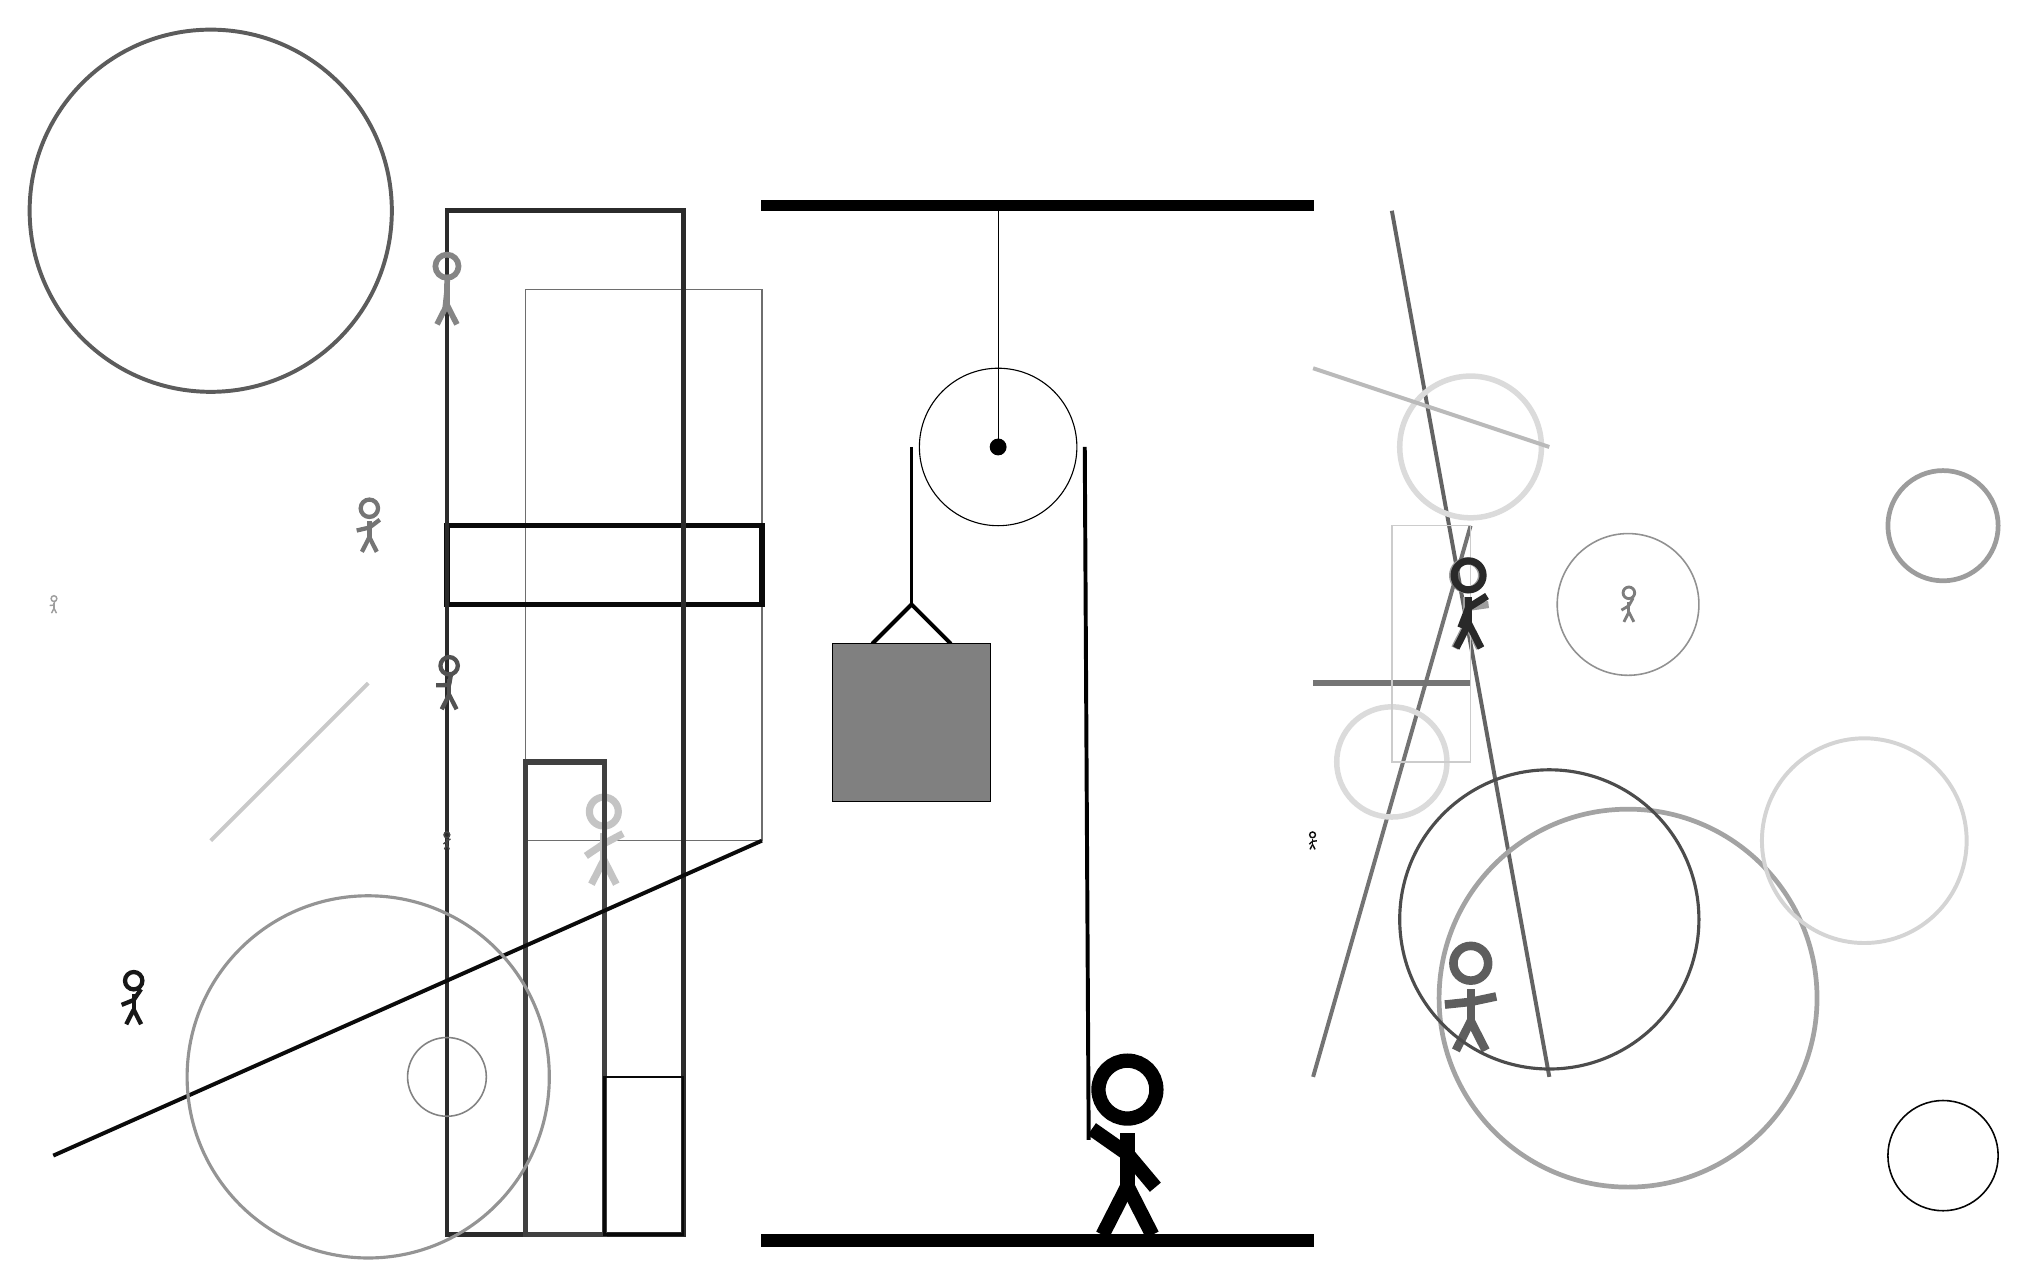
\begin{tikzpicture}
			%%%%% START %%%%%
			
			\draw[fill=black] (-2, 10) rectangle (5, 10.125);
			
			\draw (1, 7) circle (1);
			\draw[fill=black] (1, 7) circle (0.1);
			\draw (1, 10) -- (1, 7);
			
			\draw[line width=0.5mm] (-0.6, 4.5) -- (-0.1, 5.0) -- (0.4, 4.5);
			\draw[fill=black!50] (-1.1, 4.5) rectangle (0.9, 2.5);
			
			\draw[line width=0.2mm, color=black!57] (-2, 2) rectangle (-5, 9);
			
			\node[line width=0.3mm, color=black!38] at (-11, 5) {\Strichmaxerl[1][6][80]};
			\node[line width=0.6mm, color=black!94] at (5, 2) {\Strichmaxerl[1][42][6]};
			\draw [line width=0.6mm, color=black!39](13, 6) circle (0.7);
			\draw[line width=0.5mm, color=black!61](8, -1) -- (6, 10);
			\draw[line width=0.7mm, color=black!96] (-2, 6) rectangle (-6, 5);
			\node[line width=0.4mm, color=black!38] at (7, 5) {\Strichmaxerl[5][89][8]};
			\node[line width=0.3mm, color=black!63] at (7, 0) {\Strichmaxerl[6][6][12]};
			\draw[line width=0.7mm, color=black!54] (5, 4) rectangle (7, 4);
			\draw[line width=0.5mm, color=black!55](5, -1) -- (7, 6);
			\draw[line width=0.6mm, color=black!83] (-3, -3) rectangle (-6, 10);
			
			\draw [line width=0.7mm, color=black!14](7, 7) circle (0.9);
			\draw [line width=0.2mm, color=black!49](-6, -1) circle (0.5);
			
			\draw [line width=0.6mm, color=black!36](9, 0) circle (2.4);
			\draw [line width=0.2mm, color=black!98](13, -2) circle (0.7);
			\node[line width=0.7mm, color=black!23] at (-4, 2) {\Strichmaxerl[5][34][28]};
			
			\draw[line width=0.7mm, color=black!75] (-4, -3) rectangle (-5, 3);
			\draw [line width=0.2mm, color=black!43](9, 5) circle (0.9);
			\draw [line width=0.7mm, color=black!14](6, 3) circle (0.7);
			\draw[line width=0.5mm, color=black!96](-2, 2) -- (-11, -2);
			\node[line width=0.5mm, color=black!54] at (-7, 6) {\Strichmaxerl[3][13][37]};
			
			\draw [line width=0.5mm, color=black!64](-9, 10) circle (2.3);
			\node[line width=0.2mm, color=black!48] at (-6, 9) {\Strichmaxerl[4][84][89]};
			\draw[line width=0.5mm, color=black!21](-7, 4) -- (-9, 2);
			\draw[line width=0.5mm, color=black!27](8, 7) -- (5, 8);
			\draw[line width=0.3mm, color=black!97] (-4, -3) rectangle (-3, -1);
			
			\node[line width=0.2mm, color=black!73] at (-6, 2) {\Strichmaxerl[1][38][34]};
			\draw[line width=0.2mm, color=black!20] (6, 6) rectangle (7, 3);
			
			\node[line width=0.6mm, color=black!68] at (-6, 4) {\Strichmaxerl[3][1][80]};
			\draw [line width=0.4mm, color=black!42](-7, -1) circle (2.3);
			\node[line width=0.4mm, color=black!91] at (-10, 0) {\Strichmaxerl[3][22][56]};
			
			\draw [line width=0.5mm, color=black!17](12, 2) circle (1.3);
			\draw [line width=0.4mm, color=black!70](8, 1) circle (1.9);
			
			\node[line width=0.2mm, color=black!84] at (7, 5) {\Strichmaxerl[5][69][32]};
			\node[line width=0.4mm, color=black!51] at (9, 5) {\Strichmaxerl[2][31][61]};
			
			\draw[line width=0.5mm] (-0.1, 7) -- (-0.1, 5.0);
			\centerarc[line width=0.5mm](1, 7)(0:180:1.1);
			\draw[line width=0.5mm](2.1, 7) -- (2.15, -1.8);
			
			\node at (2.6, -1.9) {\Strichmaxerl[10][-35][-50]};
			
			\draw[fill=black] (-2, -3) rectangle (5, -3.15);
			
			%%%%% END %%%%%
		\end{tikzpicture}
	\end{figure}	
\end{document}